\documentclass{tufte-handout}

\usepackage{amsmath}

% Set up the images/graphics package
\usepackage{graphicx}
\setkeys{Gin}{width=\linewidth,totalheight=\textheight,keepaspectratio}
\graphicspath{{graphics/}}

\usepackage{mcaption} % FIXME move to .cls file

%\title{An Example of the Usage of the Tufte-Handout Style\thanks{Inspired by Edward~R. Tufte!}}
\title{An Example of the Usage of the Tufte-Handout Style}
\author{The Tufte-\LaTeX\ Developers}
%\date{22 February 2008}  % if the \date{} command is left out, the current date will be used

\usepackage{helvet}

% The following package makes prettier tables.  We're all about the bling!
\usepackage{booktabs}

% The units package provides nice, non-stacked fractions and better spacing
% for units.
\usepackage{units}

% The fancyvrb package lets us customize the formatting of verbatim
% environments.  We use a slightly smaller font.
\usepackage{fancyvrb}
\fvset{fontsize=\normalsize}

\usepackage{multicol}

\usepackage[savepos]{zref}

\usepackage{lipsum}

\usepackage{url}
\urldef{\asyurl}\url{http://asymptote.sf.net/}

\begin{document}

\maketitle % this prints the handout title, author, and date

\begin{abstract}
\noindent This document describes the Tufte handout \LaTeX\ document style.
It also provides examples and comments on the style's use.
\end{abstract}

%\printclassoptions

The \Verb|tufte-handout| document class defines a style similar to the
style Edward Tufte uses in his books and handouts.  Tufte's style is known
for its extensive use of sidenotes, tight integration of graphics with
text, and well-set typography.  This document aims to be at once a
demonstration of the features of the \Verb|tufte-handout| document class
and a style guide to its use.

\section{Page Layout}\label{sec:page-layout}
\subsection{Headings}\label{sec:headings}
This style provides \textsc{a}- and \textsc{b}-heads (that is,
\Verb|\section| and \Verb|\subsection|) demonstrated above.

If you need more than two levels of section headings, you'll have to define
them yourself at the moment;\sidenote{See see ``Defining new sections'' on
page~\pageref{sec:defining-sections} for help with defining more heading
levels.} there are no pre-defined styles for anything below a
\Verb|\subsection|.  As Bringhurst points out in \textit{The Elements of
Typographic Style},\cite{Bringhurst2005} you should ``use as many levels of
headings as you need: no more, and no fewer.''

The Tufte-handout class will emit an error if you try to use
\Verb|\subsubsection| and smaller headings.

%\medskip
%\begin{fullwidth}
%\begin{Verbatim}
%! Package tufte-handout Error: \subsubsection is undefined by this class.
%(tufte-handout)                See Robert Bringhurst's _The Elements of 
%(tufte-handout)                Typographic Style_, section 4.2.2. 
%(tufte-handout)                \subsubsection was used.
%\end{Verbatim}
%\end{fullwidth}
%\medskip

% let's start a new thought -- a new section
\newthought{In his later books},\cite{Tufte2006} Tufte
starts each section with a bit of vertical space, a non-indented paragraph,
and sets the first few words of the sentence in \textsc{small caps}.  To
accomplish this using this style, use the \Verb|\newthought| command:  

\Verb|\newthought{In his later books}, Tufte starts|\ldots

\subsection{Sidenotes}\label{sec:sidenotes}
One of the most prominent and distinctive features of this style is the
extensive use of sidenotes.  There is a wide margin to provide ample room
for sidenotes and small figures.  Any \Verb|\footnote|s will automatically
be converted to sidenotes.\footnote{This is a sidenote that was entered
using the \texttt{\textbackslash footnote} command.}  If you'd like to place ancillary
information in the margin without the sidenote mark (the superscript
number), you can use the \Verb|\marginnote| command.\marginnote{This is a
margin note.  Notice that there isn't a number preceding the note, and
there is no number in the main text where this note was written.}

\subsection{References}
References are placed alongside their citations as sidenotes,
as well.  This can be accomplished using the normal \Verb|\cite|
command.\footnote{The first paragraph of this document includes a citation.}

The complete list of references may also be printed automatically by using
the \Verb|\bibliography| command.  (See the end of this document for an
example.)  If you do not want to print a bibliography at the end of your
document, use the \Verb|\nobibliography| command in its place.  

To enter multiple citations at one
location,\cite{Tufte2006}\cite{Tufte1990} you will need to use multiple
\Verb|\cite| commands: \Verb|\cite{Tufte2006}| \Verb|\cite{Tufte1990}|.  Each
\Verb|\cite| command will generate its own sidenote and its own sidenote
number. 


\section{Figures and Tables}\label{sec:figures-and-tables}
Images and graphics play an integral role in Tufte's work.
In addition to the standard \Verb|figure| and \Verb|tabular| environments,
this style provides special figure and table environments for full-width
floats.

Full page width figures and tables may be placed in \texttt{figure*} or
\texttt{table*} environments.  To place figures or tables in the margin,
use the \Verb|marginfigure| or \Verb|margintable| environments as follows
(see figure~\ref{fig:marginfig}):
\begin{marginfigure}
  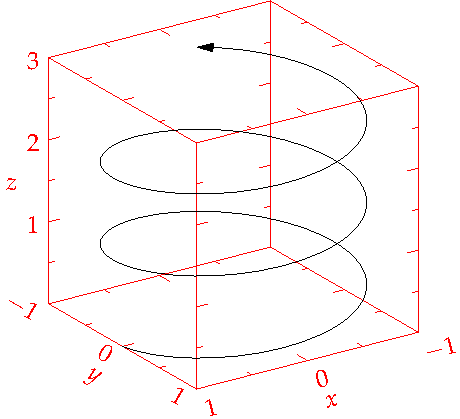
\includegraphics[width=\marginparwidth]{helix}
  \caption{This is a margin figure.  The helix is defined by 
    $x = \cos(2\pi z)$, $y = \sin(2\pi z)$, and $z = [0, 2.7]$.  The figure was
    drawn using Asymptote (\asyurl).}
  \label{fig:marginfig}
\end{marginfigure}
\begin{Verbatim}
\begin{marginfigure}
  \includegraphics{blah}
  \caption{This figure is in the margin.}
\end{marginfigure}
\end{Verbatim}


Figure~\ref{fig:fullfig} is an example of the \Verb|figure*|
environment and figure~\ref{fig:textfig} is an example of the normal
\Verb|figure| environment.
\begin{figure*}
  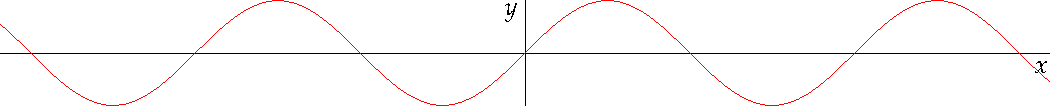
\includegraphics{sine.pdf}
  \caption{This graph shows $y = \sin x$ from about $x = [-10, 10]$.
  \emph{Notice that this figure takes up the full page width.}}
  \label{fig:fullfig}
  \zsavepos{pos:fullfig}
\end{figure*}

\begin{figure}
  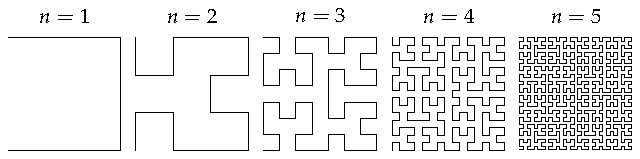
\includegraphics{hilbertcurves.pdf}
  \caption{Hilbert curves of various degrees $n$.
  \emph{Notice that this figure only takes up the main textblock width.}}
  \label{fig:textfig}
  \zsavepos{pos:textfig}
\end{figure}

Table~\ref{tab:normaltab} shows table created with the \texttt{booktabs}
package.  Notice the lack of vertical rules---they serve only to clutter
the table's data.

\begin{table}[ht]
  \centering
  \begin{tabular}{ll}
    \toprule
    Margin & Length \\
    \midrule
    Paper width & \unit[8\nicefrac{1}{2}]{inches} \\
    Paper height & \unit[11]{inches} \\
    Textblock width & \unit[6\nicefrac{1}{2}]{inches} \\
    Textblock/sidenote gutter & \unit[\nicefrac{3}{8}]{inches} \\
    Sidenote width & \unit[2]{inches} \\
    \bottomrule
  \end{tabular}
  \caption{Here are the dimensions of the various margins used in the Tufte-handout class.}
  \label{tab:normaltab}
  \zsavepos{pos:normaltab}
\end{table}

\section{Full-width text blocks}

In addition to the new float types, there is a \texttt{fullwidth}
environment that stretches across the main text block and the sidenotes
area.

\begin{Verbatim}
\begin{fullwidth}
Lorem ipsum dolor sit amet...
\end{fullwidth}
\end{Verbatim}

\begin{fullwidth}
\small\itshape\lipsum[1]
\end{fullwidth}

\section{Typography}\label{sec:typography}

\subsection{Typefaces}\label{sec:typefaces}
If the Palatino and Bera Mono typefaces are installed, this style will use
them automatically.  Otherwise, we'll fall back on the Computer Modern
typefaces.

\subsection{Letterspacing}\label{sec:letterspacing}
This document class includes two new commands and some improvements on
existing commands for letterspacing.

When setting strings of \allcaps{ALL CAPS} or \smallcaps{small caps}, the
letterspacing---that is, the spacing between the letters---should be
increased slightly.\cite{Bringhurst2005}  The \Verb|\allcaps| command has proper letterspacing for
strings of \allcaps{FULL CAPITAL LETTERS}, and the \Verb|\smallcaps| command
has letterspacing for \smallcaps{small capital letters}.  These commands
will also automatically convert the case of the text to upper- or
lowercase, respectively.

The \Verb|\textsc| command has also been redefined to include
letterspacing.  The case of the \Verb|\textsc| argument is left as is,
however.  This allows one to use both uppercase and lowercase letters:
\textsc{The Initial Letters Of The Words In This Sentence Are Capitalized.}


\section{Customization}\label{sec:customization}
\subsection{Document class options}\label{sec:options}
The \Verb|tufte-handout| class is based on the \LaTeX\ \Verb|article|
document class.  Therefore, you can pass any of the typical article
options.  There are a few options that are specific to the
\Verb|tufte-handout| document class, however.

The \Verb|a4paper| option will set the paper size to \smallcaps{A4} instead of
the default \smallcaps{US} letter size.

The \Verb|sfsidenotes| option will set the sidenotes in a \textsf{sans
serif} typeface instead of the default roman.

The \Verb|twoside| option will modify the running heads so that the page
number is printed on the outside edge (as opposed to always printing the page
number on the right-side edge in \Verb|oneside| mode).  

The \Verb|symmetric| option typesets the sidenotes on the outside edge of
the page.  This is how books are traditionally printed, but is contrary to
Tufte's book design which sets the sidenotes on the right side of the page.
This option implicitly sets the \Verb|twoside| option.

The \Verb|justified| option sets all the text fully justified (flush left
and right).  The default is to set the text ragged right.  
The body text of Tufte's books are set ragged right.  This prevents
needless hyphenation and makes it easier to read the text in the slightly
narrower column.

\subsection{Defining new sections}\label{sec:defining-sections}
As mentioned on page~\pageref{sec:headings}, the \Verb|tufte-handout|
document class only defines \Verb|\section| and \Verb|\subsection|
headings.  

If you wanted to define, say, a \Verb|\paragraph| heading, you could do it
as follows:

\begin{Verbatim}
\makeatletter
\renewcommand\paragraph{\@startsection{paragraph}% the name of the new section
  {4}% the section level number
  {0em}% indentation amount
  {\baselineskip}% amount of space to leave before heading
  {-1.5em}% amount of space to leave after heading
  {\normalfont\itshape}% style
}
\makeatother
\end{Verbatim}

Place that code in the preamble of your document and you'll now be able to use
\Verb|\paragraph|.  

For more details on defining section levels, see \textit{The \LaTeX\
Companion},\cite{Mittelbach2004} or use the \Verb|titlesec| package.


\section{Installation}\label{sec:installation}
To install the \Verb|tufte-handout| class, simply drop the
\Verb|tufte-handout.cls| file into the same directory as your \Verb|.tex|
file.

% TODO add instructions for installing it globally


\section{Support}\label{sec:support}

\subsection{Package Dependencies}\label{sec:dependencies}
The following is a list of packages that the \Verb|tufte-handout| document
class relies upon.  Packages marked with an asterisk are optional.
\begin{multicols}{2}
\begin{itemize}
  \item geometry
  \item ragged2e
  \item chngpage
  \item paralist
  \item textcase
  \item footmisc
  \item natbib and bibentry
  \item placeins
  \item caption
  \item fancyhdr 
  \item microtype*
  \item soul*
  \item palatino*
  \item beramono*
\end{itemize}
\end{multicols}

\subsection{Tufte-\LaTeX\ Website}\label{sec:website}
The website for the Tufte-\LaTeX\ packages is located at
\url{http://code.google.com/p/tufte-latex/}.  On our website, you'll find
links to our \smallcaps{svn} repository, mailing lists, bug tracker, and documentation.


\bibliography{sample-handout}
\bibliographystyle{plainnat}

%\section{Float Positions---DEBUG}
%Full figure: $x=\zposx{pos:fullfig}$, $y=\zposy{pos:fullfig}$
%Text figure: $x=\zposx{pos:textfig}$, $y=\zposy{pos:textfig}$
%Normal table: $x=\zposx{pos:normaltab}$, $y=\zposy{pos:normaltab}$

\end{document}
